\documentclass[a4paper,11pt,dvipsnames,addpoints]{exam}

\usepackage[english]{babel}
% Fonts %
\usepackage{fouriernc}
\usepackage[T1]{fontenc}

% Colors & Graphics %
\usepackage{xcolor}
\usepackage{graphicx}
\graphicspath{ {exam_figs/} }

% Tikz
\usepackage{tikz}
\usetikzlibrary{patterns}
\usepackage{tkz-euclide}

% Figures
\usepackage{float}
\usepackage{caption}
\usepackage{subcaption}

% Page Layout %
\usepackage[margin=1in]{geometry}

\pagestyle{headandfoot}
\firstpageheader{}{}{}
\runningfooter{}{}{}
\runningheader{Exam B}{Page~\thepage~of~\numpages}{November 26, 2024}
\runningheadrule

% Math stuff %
\usepackage{amsmath}
\usepackage{amssymb}

% Fancy Headers %
\usepackage{enumitem}

% Tables %
\usepackage{booktabs}
\usepackage{tabularx}

\newcommand{\clr}{\textcolor{BrickRed}}
\newcommand{\clb}{\textcolor{RoyalBlue}}
\newcommand{\clg}{\textcolor{ForestGreen}}
\newcommand{\clf}{\textcolor{Fuchsia}}

% Rename solution
\setlength{\fboxsep}{8pt}

% Document %
\begin{document}
\marginpointname{~\%}
\bracketedpoints
\pointsinrightmargin

\begin{center}
 \Huge\sffamily Convex Polygons and Their Symmetries\\[4pt]
 \Large\sffamily 3.AB PreIB Maths -- Exam B
\end{center}

\begin{center}
\framebox{%
 \parbox{.7\textwidth}{%
  \centering
  Unless specified otherwise, you are to \textbf{\clr{always}} (at least
  briefly) explain your reasoning. Even in closed questions.
 }
}
\end{center}
\begin{questions}
 \question Definition of a polygon.
 \begin{parts}
  \part[10] Which of these shapes \emph{\clr{are not}} polygons?
  \textbf{Explain}.
  \begin{figure}[H]
   \centering
   \begin{subfigure}[b]{.2\textwidth}
    \centering
    \includegraphics[width=\textwidth]{not_poly_1}
    \caption*{Option A.}
   \end{subfigure}
   \hfill
   \begin{subfigure}[b]{.2\textwidth}
    \centering
    \includegraphics[width=\textwidth]{poly_1}
    \caption*{Option B.}
   \end{subfigure}
   \hfill
   \begin{subfigure}[b]{.2\textwidth}
    \centering
    \includegraphics[width=\textwidth]{poly_2}
    \caption*{Option C.}
   \end{subfigure}
   \hfill
   \begin{subfigure}[b]{.2\textwidth}
    \centering
    \includegraphics[width=\textwidth]{not_poly_2}
    \caption*{Option D.}
   \end{subfigure}
  \end{figure}
  \vspace{2in}
  \part[10] Try to count the number of pairs of \emph{\clr{parallel}} diagonals
  in a \textbf{regular} polygon on $n$ vertices. For example, the hexagon has
  three such pairs:
  \begin{figure}[H]
   \centering
   \begin{subfigure}[b]{.3\textwidth}
    \centering
    \includegraphics[width=.5\textwidth]{hexa_parallel_1}
   \end{subfigure}
   \begin{subfigure}[b]{.3\textwidth}
    \centering
    \includegraphics[width=.5\textwidth]{hexa_parallel_2}
   \end{subfigure}
   \begin{subfigure}[b]{.3\textwidth}
    \centering
    \includegraphics[width=.5\textwidth]{hexa_parallel_3}
   \end{subfigure}
  \end{figure}
  \textbf{Hint:} Distinguish polygons with even number of vertices from those
  with odd.
  \clearpage
 \end{parts}

 \question Triangulations of convex polygons.
 \begin{parts}
  \part[10] Draw all triangulations of the pentagon \emph{\clr{that can be
  reached in one flip}} from the one shown below. Use the provided shapes (not
  all of them necessarily). \textbf{No explanation required}.
  \begin{figure}[H]
   \centering
   \includegraphics[width=.15\textwidth]{penta_triangulation}

   \caption*{The initial triangulation.}
  \end{figure}
  \begin{figure}[H]
   \centering
   \begin{subfigure}[b]{.3\textwidth}
    \centering
    \includegraphics[width=.5\textwidth]{penta_plain}
   \end{subfigure}
   \begin{subfigure}[b]{.3\textwidth}
    \centering
    \includegraphics[width=.5\textwidth]{penta_plain}
   \end{subfigure}
   \begin{subfigure}[b]{.3\textwidth}
    \centering
    \includegraphics[width=.5\textwidth]{penta_plain}
   \end{subfigure}
  \end{figure}
  \begin{figure}[H]
   \centering
   \begin{subfigure}[b]{.3\textwidth}
    \centering
    \includegraphics[width=.5\textwidth]{penta_plain}
   \end{subfigure}
   \begin{subfigure}[b]{.3\textwidth}
    \centering
    \includegraphics[width=.5\textwidth]{penta_plain}
   \end{subfigure}
   \begin{subfigure}[b]{.3\textwidth}
    \centering
    \includegraphics[width=.5\textwidth]{penta_plain}
   \end{subfigure}
   \caption*{Shapes to draw diagonals into.}
  \end{figure}
  \part[10] Can every \emph{\clr{non-convex}} polygon also be triangulated, that
  is, divided into triangles by non-intersecting diagonals? Try to think of an
  argument or provide a counterexample. 
  \begin{figure}[H]
    \centering
    \includegraphics[width=.2\textwidth]{non_convex_hexa_triangulation}
    \caption*{A \clr{triangulation} of a non-convex hexagon.}
   \end{figure}
  \end{parts}
 \clearpage
 \question Plane transformations.
 \begin{parts}
  \part[10] Find out the \emph{\clg{image}} (the resulting shape when
  transformed) of a square (depicted below) under the plane transformation
  $\clb{f}(x,y) = (x,y-x)$. \textbf{Provide a short explanation}.
  \begin{figure}[H]
   \centering
   \begin{subfigure}[c]{.3\textwidth}
    \centering
    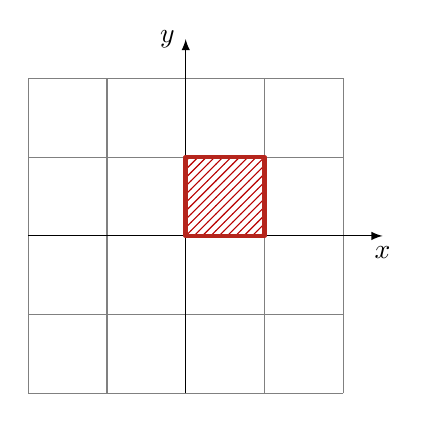
\begin{tikzpicture}
     \tkzInit[xmin=-2,xmax=2,ymin=-2,ymax=2]
     \tkzGrid
     \tkzDrawX
     \tkzDrawY
     \tkzDefPoints{0/0/a,0/1/b,1/1/c,1/0/d}
     \tkzDrawPolygon[ultra thick,BrickRed,pattern={north east lines}, pattern
     color=BrickRed](a,b,c,d)
    \end{tikzpicture}
    \caption*{The initial \clr{square}.}
   \end{subfigure}
   \hspace*{-2em}
   \begin{subfigure}[b]{.3\textwidth}
    \centering
    \begin{tikzpicture}
     \node (origin) at (0,0) {};
     \draw[-latex,thick,bend left=30,RoyalBlue] (0,1) to
      node[midway,yshift=3mm]{$f$} (4,1);
    \end{tikzpicture}
   \end{subfigure}
   \begin{subfigure}[c]{.3\textwidth}
    \centering
    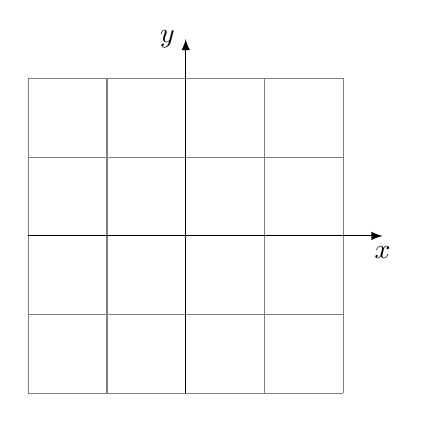
\begin{tikzpicture}
     \tkzInit[xmin=-2,xmax=2,ymin=-2,ymax=2]
     \tkzGrid
     \tkzDrawX
     \tkzDrawY
    \end{tikzpicture}
    \caption*{Draw the resulting shape here.}
   \end{subfigure}
  \end{figure}
  \vspace{2in}
  \part[10] Below, you see a unit \clr{square} transformed by the plane
  transformation $\clg{f}$. The function $\clg{f}$ sends the $x$-coordinate of
  every point to $1 - y + 2x$. What does it send the $y$-coordinate to?
  \textbf{Explain}.
  \begin{figure}[H]
   \centering
   \begin{subfigure}[c]{.35\textwidth}
    \centering
    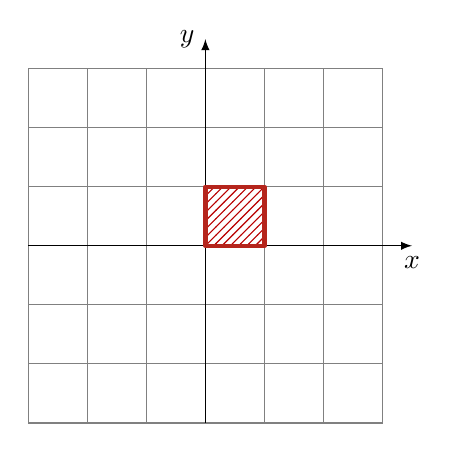
\begin{tikzpicture}[scale=0.75]
     \tkzInit[xmin=-3,xmax=3,ymin=-3,ymax=3]
     \tkzGrid
     \tkzDrawX
     \tkzDrawY
     \tkzDefPoints{0/0/a,0/1/b,1/1/c,1/0/d}
     \tkzDrawPolygon[ultra thick,BrickRed,pattern={north east lines}, pattern
     color=BrickRed](a,b,c,d)
    \end{tikzpicture}
    \caption*{The \clr{initial} square.}
   \end{subfigure}
   \hspace*{-2em}
   \begin{subfigure}[b]{.2\textwidth}
    \centering
    \begin{tikzpicture}
     \node (origin) at (0,0) {};
     \draw[-latex,thick,bend left=30,ForestGreen] (0,1) to
      node[midway,yshift=3mm]{$f$} (3,1);
    \end{tikzpicture}
   \end{subfigure}
   \begin{subfigure}[c]{.35\textwidth}
    \centering
    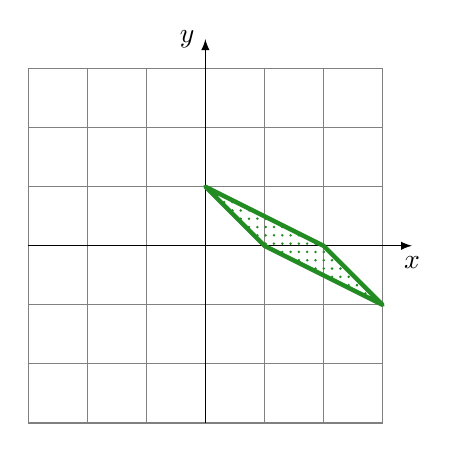
\begin{tikzpicture}[scale=0.75]
     \tkzInit[xmin=-3,xmax=3,ymin=-3,ymax=3]
     \tkzGrid
     \tkzDrawX
     \tkzDrawY
     \tkzDefPoints{1/0/a,3/-1/b,2/0/c,0/1/d}
     \tkzDrawPolygon[ultra thick,ForestGreen,pattern={dots}, pattern
     color=ForestGreen](a,b,c,d)
    \end{tikzpicture}
   \caption*{The square transformed by $\clg{f}$.}
   \end{subfigure}
  \end{figure}
 \end{parts}
 \clearpage
 \question Symmetries of regular polygons.
 \begin{parts}
  \part[10] Given two symmetries of the \emph{square} -- the rotation $\clr{r} =
  ~\circlearrowleft 90^{ \circ }$ by $90^{ \circ }$ counter-clockwise and the
  reflection $\clb{s}$ drawn below -- determine (using any method you wish) the
  composition $\clr{r}\clb{s}$. \textbf{Explain}.
  \begin{center}
   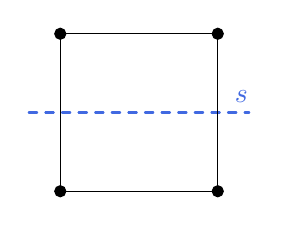
\begin{tikzpicture}[scale=2]
    \tkzInit
    \tkzDefPoints{0/0/a,0/1/b,1/1/c,1/0/d}
    \tkzDefMidPoint(a,b)\tkzGetPoint{m1}
    \tkzDefMidPoint(c,d)\tkzGetPoint{m2}
    \tkzDrawLine[thick,dashed,RoyalBlue](m1,m2)
    \tkzLabelLine[pos=1.2,yshift=2mm,xshift=-1mm](m1,m2){$\clb{s}$}
    \tkzDrawPoints[size=4,fill=black](a,b,c,d)
    \tkzDrawPolygon(a,b,c,d)
   \end{tikzpicture}
  \end{center}
  \vspace{2in}
  \part[10] Given two symmetries of the icosiheptagon (27 vertices) -- the
  reflections $\clr{s_1}$ and $\clb{s_2}$ depicted below -- compute (using any
  method you wish) the composition $\clb{s_2}\clr{s_1}$. \textbf{Explain}.
  \begin{figure}[H]
   \centering
   \begin{tikzpicture}[scale=3]
    \tkzInit
    \foreach \n/\a in
    {1/0.0, 2/13.333333333333334, 3/26.666666666666668, 4/40.0,
     5/53.333333333333336, 6/66.66666666666667, 7/80.0, 8/93.33333333333334,
     9/106.66666666666667, 10/120.0, 11/133.33333333333334, 12/146.66666666666669,
     13/160.0, 14/173.33333333333334, 15/186.66666666666669, 16/200.0,
     17/213.33333333333334, 18/226.66666666666669, 19/240.0, 20/253.33333333333334,
     21/266.6666666666667, 22/280.0, 23/293.33333333333337, 24/306.6666666666667,
     25/320.0, 26/333.33333333333337, 27/346.6666666666667}
    {%
     \tkzDefPoint(\a:1){\n}
    }
    \foreach \n in {1,2,...,27}{%
     \tkzDrawPoint[size=4,fill=black](\n)
    }
    \tkzDefMidPoint(8,9)\tkzGetPoint{m1}
    \tkzDefMidPoint(25,26)\tkzGetPoint{m2}
    \tkzDrawLine[thick,dashed,RoyalBlue](22,m1)
    \tkzDrawLine[thick,dashed,BrickRed](12,m2)
    \tkzLabelLine[pos=1.2,yshift=-1mm,xshift=3mm](22,m1){$\clb{s_2}$}
    \tkzLabelLine[pos=1.2,yshift=3mm,xshift=-1mm](12,m2){$\clr{s_1}$}
    \tkzDrawPolygon(1,2,3,4,5,6,7,8,9,10,11,12,13,14,15,16,17,18,19,20,21,22,23,24,25,26,27)
   \end{tikzpicture}
  \end{figure}
  \clearpage
  \part[10] Select those of the following four pairs of symmetries of the
  regular hendecagon (11 vertices) that \emph{\clr{generate all}} of its
  symmetries. \textbf{No explanation necessary}.
  \begin{figure}[H]
   \centering
   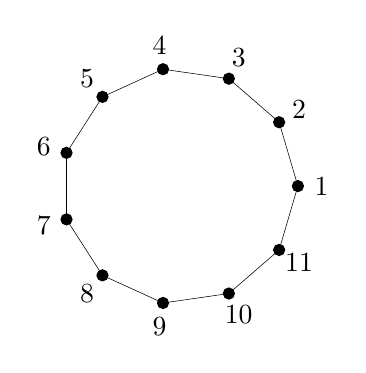
\begin{tikzpicture}[scale=1.5]
    \foreach \n/\a in {
     1/0.0, 2/32.72727272727273, 3/65.45454545454545, 4/98.18181818181819,
     5/130.9090909090909, 6/163.63636363636363, 7/196.36363636363637,
     8/229.0909090909091, 9/261.8181818181818, 10/294.54545454545456,
     11/327.27272727272725
     } {
      \tkzDefPoint(\a:1){\n}
      \tkzDrawPoint[size=4,fill=black](\n)
      \node at (\a:1.2) {$\n$};
     }
     \tkzDrawPolygon(1,2,3,4,5,6,7,8,9,10,11)
   \end{tikzpicture}
   \caption*{Picture of the hendecagon for reference.}
  \end{figure}
  \begin{checkboxes}
   \item the reflection $\clb{s}$ over the line passing through vertex $1$ and
    the midpoint of $67$ and the rotation $\clr{r} = ~\circlearrowleft 3 \cdot
    360^{ \circ } / 11$,
   \item the rotation $\clr{r_1} =~\circlearrowleft 5 \cdot 360^{ \circ } / 11$
    and the rotation $\clr{r_2} = ~\circlearrowleft 7 \cdot 360^{ \circ } / 11$,
   \item the rotation $\clr{r} =~\circlearrowleft 7 \cdot 360^{ \circ } / 11$ and
    the reflection $\clb{s}$ over the line passing through vertex $4$ and the
    midpoint of $9,10$,
   \item the reflection $\clb{s_1}$ over the line passing through vertex $2$ and
    the midpoint of $78$ and the reflection $\clb{s_2}$ over the line passing
    through vertex $3$ and the midpoint of $89$.
  \end{checkboxes}
  \part[10] Given reflections $\clr{s_1}$ and $\clb{s_2}$ of the octagon (8
  vertices), compose them (and \emph{\clr{only}} them) to create the reflection
  $\clg{s_3}$ illustrated below. \textbf{Explain}.
  \begin{center}
   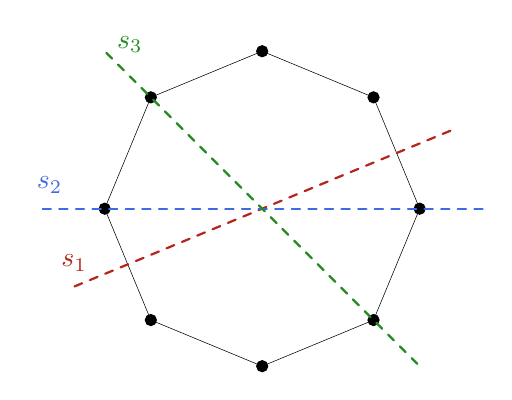
\begin{tikzpicture}[scale=2]
    \foreach \n/\a in {
      1/0.0, 2/45.0, 3/90.0, 4/135.0, 5/180.0, 6/225.0, 7/270.0, 8/315.0
     } {
      \tkzDefPoint(\a:1){\n}
      \tkzDrawPoint[size=4,fill=black](\n)
     }
     \tkzDrawPolygon(1,2,3,4,5,6,7,8)
     \tkzDefMidPoint(1,2)\tkzGetPoint{m1}
     \tkzDefMidPoint(5,6)\tkzGetPoint{m2}
     \tkzDrawLine[thick,dashed,BrickRed](m1,m2)
     \tkzDrawLine[thick,dashed,RoyalBlue](1,5)
     \tkzLabelLine[pos=1.2,yshift=3mm](m1,m2){$\clr{s_1}$}
     \tkzLabelLine[pos=1.2,yshift=3mm,xshift=1mm](1,5){$\clb{s_2}$}

     \tkzDrawLine[thick,dashed,ForestGreen](4,8)
     \tkzLabelLine[pos=1.2,xshift=3mm,yshift=1mm](8,4){$\clg{s_3}$}
   \end{tikzpicture}
  \end{center}
 \end{parts}
\end{questions}

\end{document}
